\documentclass[letterpaper]{article}
\usepackage{aaai}
\usepackage{graphicx,curves}
\usepackage{float}
\usepackage{listings}
\title{Organic Horde}
\date{2017-03-27}
\author{David Quail\\
Department of Computing Science \\ University of Alberta \\
Edmonton, Alberta, T6G 2E8, Canada \\
dquail@ualberta.ca}
\begin{document}
\maketitle
\begin{abstract}
General value functions (GVFs) have proven to be effective in answering predictive questions about the future. However, simply answering a single predictive question has limited utility. Others have demonstrated further utility by using these GVFs to dynamically compose more abstract questions \cite{representingknowledge}, or to optimize control \cite{modayil2014prediction}. In other words, to feed the prediction back into the system. But these demonstrations have relied on a static set of GVFs, handcrafted by a human designer.

In this paper, we look to extend the Horde architecture \cite{sutton2011horde} to not only feed the GVFs back into the system, but to do so dynamically. In creating a dynamic horde, we explore ways to control the lifecycle of GVFs contained in a Horde - mainly to create, test, cull, and recreate GVFs, in an attempt to maximize some objective.
\end{abstract}
    
\section{Background}

General value functions are an adaptation of conventional value functions in an effort to represent predictive knowledge. These GVFs have the ability to learn from continuous valued inputs, such as those from robots. The goal of a GVF is not to maximize a specific reward signal, but rather to predict its value. In addition to the specific goal of representing predictive knowledge, GVFs differ from conventional value functions from Reinforcement Learning in two implementation differences we will discuss.
First, rather than a reward that is being measured, each GVF is predicting a certain ``cumulant'' value z. The agent is not attempting to maximize this cumulant, unlike the reward. The main concern is to predict the future cumulant, rather than to maximize it. Secondly, ``termination'' is handled much differently with GVFs than conventional value functions. In the latter case, $\gamma$ is a discount factor that weights the value of future rewards. By changing $\gamma$ the designer is deciding how much future rewards are worth, in comparison to immediate rewards. This is also the case with a GVF, however, in the case of GVFs this $\gamma$ is state dependent, thus allowing the timescale of the prediction to be sculpted. For example, a robot attempting to predict the number of steps to a wall, could have a $\gamma$ of 1.0 for every state other than the one where it's at the wall. When at the wall, $\gamma$ = 0.0. In this way, the cumulant predicts the exact number of steps to the wall, and then ``terminates'' the prediction once there.

GVFs defined this way have demonstrated a compact way to express knowledge \cite{littman2002predictive}. But in and of themselves, don't prove any value to an actual agent. They don't feed back into the system to provide further value. In an agent architecture, they seem to be off on the side, un-used by the rest of the system.

One fairly intuitive vision of how these GVFs may integrate with the reset of a learning system, is that they form a rich ecosystem of integrated GVFs. Each GVF may feed into another, to create topologies of GVFs. Lower level GVFs are the input into other higher level GVFs which answer more abstract questions, or optimize the control of the agent. One could imagine a networked ecosystem of tens of thousands of GVFs, The strongest, most useful GVFs continue to survive, while the useless and week ones are recycled for new candidate GVFs. The resulting GVF network would be helping more accurately and efficiently predict higher level questions, or optimizing control. We refer to such a system of GVFs as a ``dynamic'' or ``organic'' horde'.

An ecosystem of GVFs is not only intuitively promising, but also demonstrably useful. Mark Ring's thought experiments \cite{representingknowledge} clearly articulate how lower level GVFs based on raw sensorimotor data could be used to create more abstract GVFs. 

Litman and Sutton demonstrated that predictive representation of state can be effective in partially observable Markov decision processes \cite{littman2002predictive}. And Sutton and Pilarski demonstrated an ability to create tens of thousands of GVFs (demons) making predictions in parallel \cite{sutton2011horde}. Therefore, such a system of dynamic GVFs seems very attainable. 

There are obviously several challenges and questions remaining before building such a system. What actually makes a ``good'' GVF? How do you test and measure this ``goodness?'' How do you create GVFs dynamically in an optimal way? Which GVFs should should be destroyed? And when?

We look to start answering these GVF lifecycle questions in this research project.


\section{Experimental Setup}
In order to start answering these questions, we looked for an experimental setup that would provide a continuous stream of low level sensory data, allowing us to make many predictions from the data. From this stream of data we would be able to create numerous possible GVFs (demons) that could feed into a single higher level GVF. The prediction accuracy of this higher level GVF would be our measure of how effective our organic horde was at generating useful GVFs. In our experiment, we will have a layer of GVFs providing their output to a higher level predictor unit. This higher level unit will use the GVFs input and the true speed to learn a model which predicts a speed at any timestep. This setup is explained in detail in later sections..

\subsection{Goals}
Ultimately, the goal is to create a horde of dynamic GVFs, able to generate useful GVFs on its own. This paper takes a step towards realizing that goal by proposing solutions and demonstrating progress in answering the following questions.
\begin{itemize}
  \item How do you create GVFs in a dynamic way?
  \item When do you decide to cull GVFs?
  \item Which GVFs should be removed?
\end{itemize}

For each of these questions, we examined and measured a few alternative approaches and measured the performance using our experimental setup as described above..

\subsection{Dynamixel setup}
To create a datastream in our experiments, we used a single Dynamixel AX-12 servo that rotated back and forth, producing an encoder position and speed at a 10Hz frequency. At any point, the actuators encoder position will produce a value between 510 and 1023 and either moving left or right. A simple form of coarse coding was used to approximate these states. The encoder space was divided into 10 different regions, and for each, the actuator may be moving left or right. Therefore, the states are approximated by a vector of 20 bits where each element is 0 except for the active state. 


\begin{figure}[H]
  \centerline{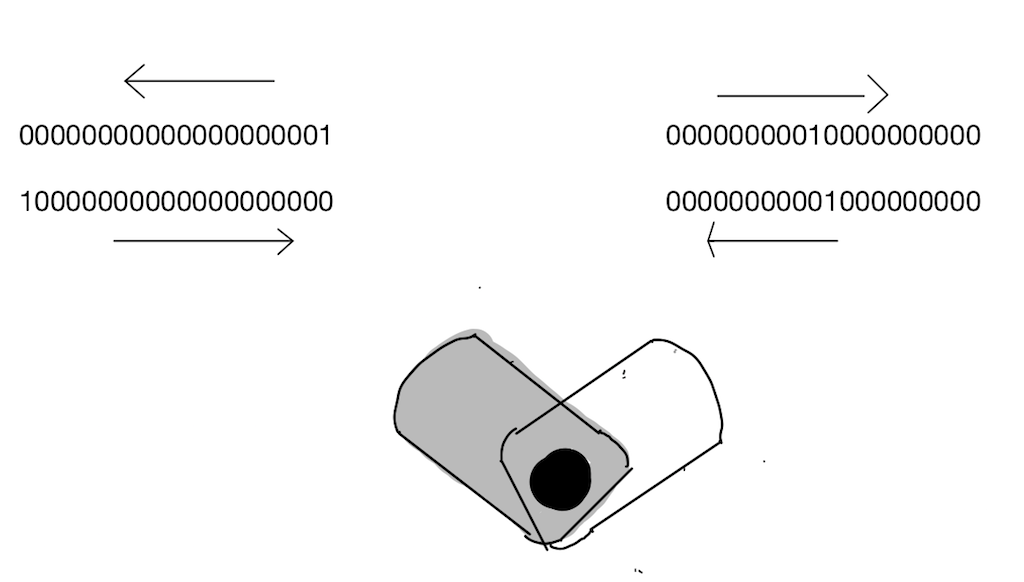
\includegraphics[width=0.5\textwidth]{Images/DynamixelFeatures.png}}
  \caption{Dynamixel state representation.}
  \label{fig:dynamixel}
\end{figure}

\subsection{Feature representation and GVF layers}
At each timestep, a feature representation is generated from the sensorimotor information as described above. This forms a vector of bits with a length of 20. In addition to these legitimate 20 bits, we add 20 bits of ```noise,'' where the value is randomly either 0 or 1. Therefor, each state is represented by a vector 40 bits in length. The first 20 bits contain information that can be learned, while the last 20 bits are purely noise. 

\begin{figure}[H]
  \centerline{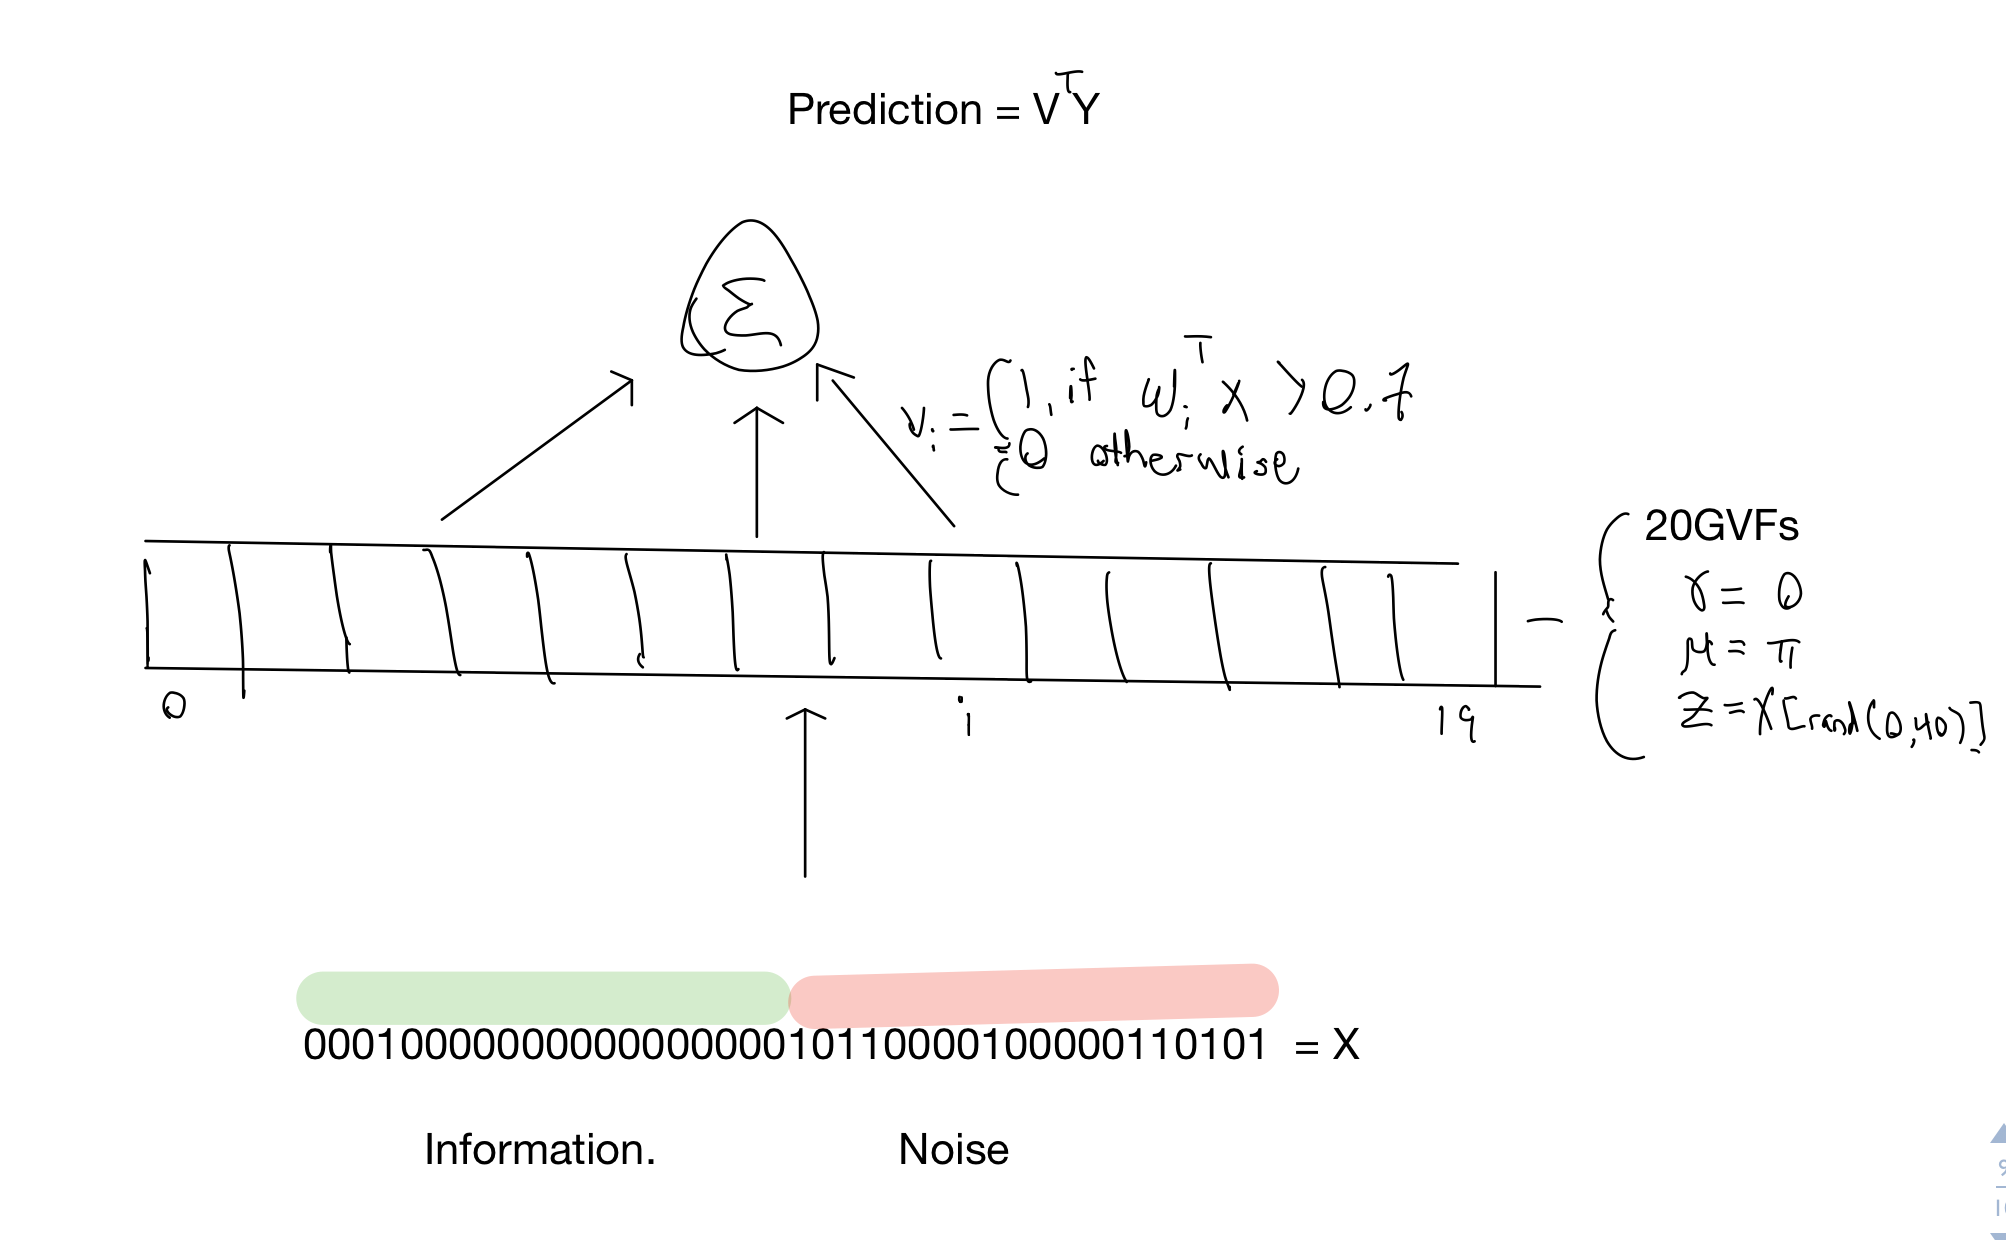
\includegraphics[width=\linewidth]{Images/ExperimentSetup.png}}
  \caption{Experimental setup}
  \label{fig:experiment}
\end{figure}

These features X are input into a layer of 20 GVFs. Each GVF is configured in such a way as to predict what the next bit will be for one of the 40 bits in the feature vector. Throughout a GVFs lifetime, it continues to predict the same bit. This is done by setting $\gamma$ = 0.0, and setting the cumulant to be one of the bits from the feature vector. It is easy to see that if the GVFs were manually chosen wisely, there would be one GVF for each bit containing information. However, in our setup, given that the GVF layer is unaware of which bits are noise and which are not, there is no obvious way for the system to select bits containing information. An alternative to this approach would have been to increase the number of GVFs in our horde, and expand on the ways to generate GVFs. For example, include different possible $\gamma$ values between 0 and 1.0. However, constraining it to 20 GVFs makes the experiment and ideal results conceptually clear. In the ideal scenario, our horde contains one GVF for each of the 20 bits actually containing information. Our system is constrained to perform no better.

Each GVF is updated using the TDLambda algorithm

\begin{lstlisting}
def tdLearn(self, lastState, newState):
  #Get the cumulant and lambda values
  zNext = self.cumulant(newState)  
  #returns bit value
  gammaNext = self.gamma(newState) 
  #always returns 0
  lam = self.lam(newState) 
  #always returns 0.95

  #Update weights
   self.eligibilityTrace = self.gammaLast 
   * lam * self.eligibilityTrace + lastState
    tdError = zNext + gammaNext * 
    numpy.inner(newState, self.W) 
     - numpy.inner(lastState, self.W)
    self.W = self.W + self.alpha * 
    tdError * self.eligibilityTrace
    self.gammaLast = gammaNext
\end{lstlisting}

The output V from the GVF is made binary by outputting a 1 if the value is greater than a threshold value of 0.7, and 0 otherwise. 

\begin{lstlisting}
GVF(X) = 1 if X^T W  > 0.7
GVF(X) = 0 otherwise
\end{lstlisting}

Finally, the output of the GVFs, along with the actual speed y, are input into the final output layer which is used to predict the speed for any state. This final layer has a set of weights Y, where each weight corresponds to one of the GVF inputs V. This layer uses a one step TD update to maintain its weights.

\begin{lstlisting}
def learn(self, X, y):
    #y is the actual value to learn from
    #X is the inputs from the 20 GVFs
    tdError = y - self.prediction(X)
    self.Y = self.Y + 
    self.alpha*tdError*X
\end{lstlisting}

\subsection{Basic algorithm}
Now that our basic configuration is established, we are able to start making predictions given a layer of GVFs. However, the setup is thus far static, much like the original Horde architecture. Our intention is to have our horde of demons organically remove the weak performers and replace with new GVFs. Therefore, we have a general algorithm such as the following 
\begin{lstlisting}
Repeat forever:
	observe new state
	foreach gvf in horde.gvfs:
		gvf.update
	if (time to cull)
		delete weakest(horde.gvfs)
		horde.gvfs.append(random(GVF))
\end{lstlisting}	

\section{Experiments}
Using this basic setup and algorithm, our intention is to conduct a number of experiments where different approaches culling and regenerating GVFs are used. For each experiment, the prediction error at each of 120,000 timesteps is averaged across 1000 runs. Comparing these averages will give us some guidance as to the effectiveness of different approaches for culling and regenerating GVFs. 

Since we know the ideal set of GVFs, we are able to measure the optimal performance of our system by manually locking in the 20 GVFs that we know represent predictions for the 20 bits actually containing information. Therefor, each of our different approaches to dynamically creating 20 GVFs can be measured against this optimal performance.


\begin{figure}[H]
  \centerline{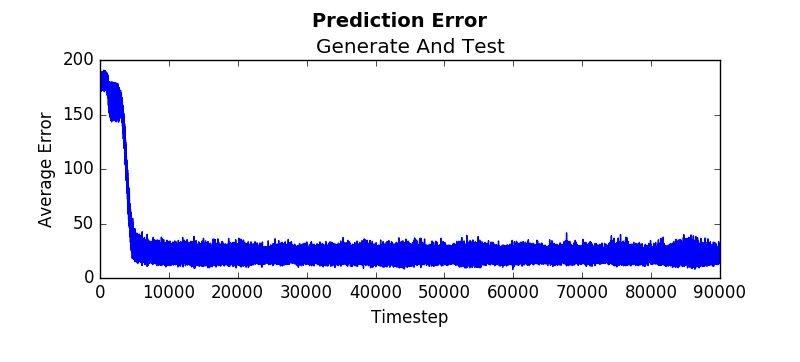
\includegraphics[width = \linewidth]{Plots/AverageErrorBestPossibleWith20RealGVFS.png}}
  \caption{Best possible learning rate with ideal 20 GVFs. Averaged across 1000 runs}
  \label{fig:ideal}
\end{figure}

\subsection{Experiment 1 - Never replace any GVFs}
The first experiment conducted, which establishes a baseline for other strategies, is to measure the performance of a system that initializes 20 random GVFs but does not change them over time. In other words, no further culling and replacing takes place.  

\subsubsection{Results}

The error decreases quickly, as there are some states which are able to make accurate predictions. However, No further reduction in error is seen over time. 

\begin{figure}[H]
  \centerline{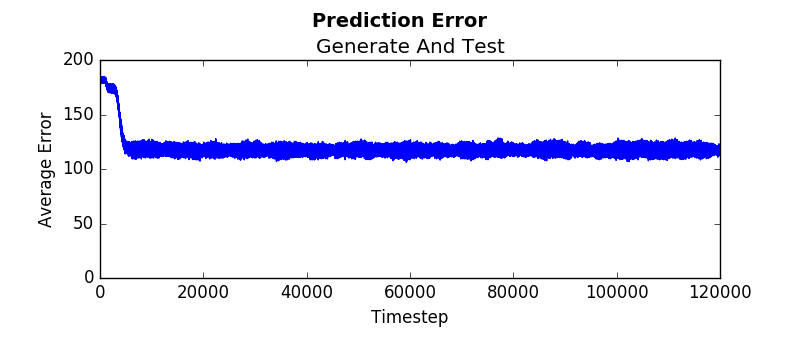
\includegraphics[width = \linewidth]{Plots/AverageErrorNoKulling.png}}
  \caption{Results without any GVF culling. Averaged across 1000 runs}
  \label{fig:experiment}
\end{figure}

\subsection{Experiment 2 - Replace weakest GVF with new Random GVF}
For this experiment, at every 5000 timesteps, we replace the weakest performing GVF (as measured by the one with the smallest absolute value weight) with a randomly chosen GVF. This newly selected GVF could be predicting something exactly the same as a current or past GVF. The intuition behind using the weights as an indicator for a GVFs utility is fairly straight forward. If a GVFs corresponding weight is low, it means it's input value is not factored into the higher level prediction, and therefor not all that useful to the prediction. 

\subsubsection{Results}

\begin{figure}[H]
  \centerline{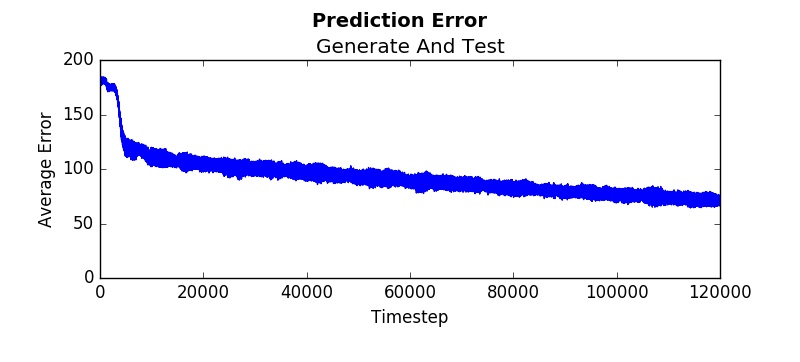
\includegraphics[width = \linewidth]{Plots/AverageErrorKullEvery5000ReplaceRandomIncludingRepeats.png}}
  \caption{Cull every 5000 time steps and replace with random GVFs. Averaged across 1000 runs}
  \label{fig:experiment}
\end{figure}	

As seen, the average error takes a significant dip as the initial GVFs are learned, and then steadily decreases over the lifetime of the horde as more proper GVFs are created. 

\subsection{Experiment 3 - Replace weakest GVF with novel GVF}
This experiment was exactly the same as Experiment 2 above with one difference. A second GVF predicting the same bit as another GVF could not be created unless all other possible GVFs had been already created. In otherwords, the regenerate step prevents the generation of GVFs that have already been created. In our experimental setup, this means that the same bit can only be predicted once by one GVF. Given this criteria, our learning rate is slightly faster given that there's no chance of us learning redundant information. After 120,000 timeteps, the average error with a strategy to create only novel GVFs is ~50; while the average error when creating random GVFs is ~75.
\subsubsection{Results}
The learning rate was faster than when choosing random, possibly repeating GVFs 

\begin{figure}[H]
  \centerline{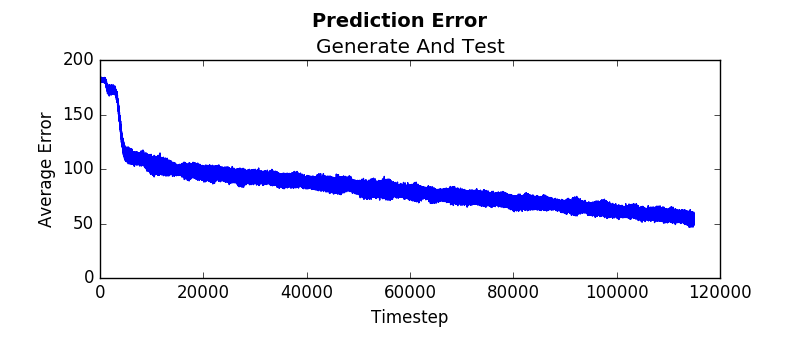
\includegraphics[width = \linewidth]{Plots/AverageErrorKullEvery500011000Steps1000Runs.png}}
  \caption{Cull every 5000 time steps and replace with novel GVFs. Averaged across 1000 runs}
  \label{fig:experiment}
\end{figure}

\section{Conclusions}
The main contribution of this paper is a demonstration that an organic Horde can indeed improve the performance of an intelligent agent by generating, testing, and regenerating GVFs in some computational way. Although the strategies were simple, we showed different rates of learning depending on when to cull, and what to replace with. This is encouraging since others have demonstrated the power and utility of GVFs, and a more organic Horde not only removes a human designer, but potentially makes the system robust in non stationary environments. 
\section{Future work}
In this paper, the methods for which these GVFs are destroyed and regenerated are intentionally not overly sophisticated as the main goal is to show such a dynamic system may exist and improve performance over time without a designer intervening. Given that the methods for which these GVFs are destroyed and regenerated are simple, a possible next step may be to further optimize how GVFs are destroyed, and regenerated. One could easily imagine exploring:
\begin{itemize}
  \item Picking GVFs based on the proximity of other ``similar'' GVFs. Radial functions could be used to define some measure of closeness. To do so, we would have to change the experimental setting here, since the distribution of GVFs is entirely random. 
  \item Picking GVFs based on following some performance gradient. What this gradient is, is completely unclear.  
  \item The best performance that we see in our experiments picking the ideal 20 GVFs still includes error and does not converge to zero. This is because that the predicted next state for some of the encoder positions is unclear. For some of these states, the usual ``next'' state is unpredictable. Therefor, these GVFs never activate, and never provide information to the higher level predictor. One idea to get around this would be including different step sizes for candidate GVFs - rather than just different prediction bits. In this way, although the next state may be unpredictable, the state in 5 timesteps might be entirely predictable. 
  \item Culling GVFs based on a combination of age and RUPEE. I considered only culling GVFs that were of a certain age AND had a certain RUPEE error. However, it's not clear that using RUPEE error as an indicator of a GVFs readiness to be culled contributes anything. I tracked RUPEE for each GVF, the GVFs that were predicting non noisy bits were relatively lower than noisy bits. So there's some motivation to using RUPEE as a measure of GVF goodness rather than it's readiness to be considered for culling.
  \item Changing the experimental configuration such that the GVFs are used to shape the feature representation, which is then used as input into another GVF whose performance is to be maximized.
  \item Using step size adaptation to determine which GVFs are good, rather than just their weights.
  \item Demonstrate the effectiveness of an organic Horde in some non-stationary experimental setting where ``good'' GVFs may change over time, further emphasizing the need for GVF creation to be \cite{White:2015} dynamic.
\end{itemize}

\section{Experimental code}
All code necessary, as well as further documentation can be found at http://github.com/dquail/RLGenerateAndTest

\bibliographystyle{aaai}
\bibliography{bibliography}
\end{document}